{\footnotesize 
\csvreader[
    tabular={cccccccccc}, % Adjust according to your table's structure
    table head={
        & % Add an empty cell for the new column
        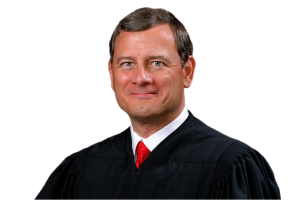
\includegraphics[width=1.5cm]{Figures/justice_images/Roberts.png} &
        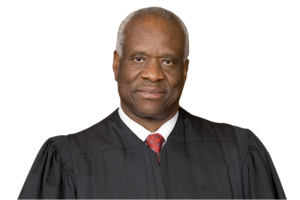
\includegraphics[width=1.5cm]{Figures/justice_images/Thomas.png} &
        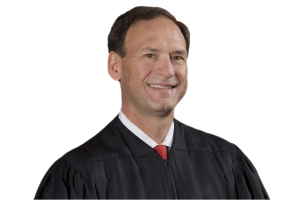
\includegraphics[width=1.5cm]{Figures/justice_images/Alito.png} &
        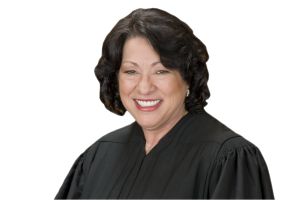
\includegraphics[width=1.5cm]{Figures/justice_images/Sotomayor.png} &
        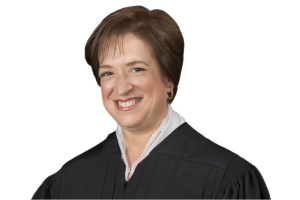
\includegraphics[width=1.5cm]{Figures/justice_images/Kagan.png} &
        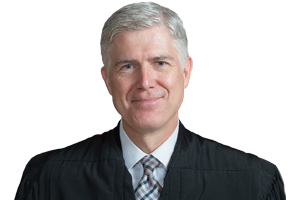
\includegraphics[width=1.5cm]{Figures/justice_images/Gorsuch.png} &
        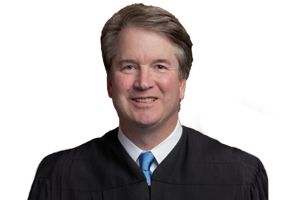
\includegraphics[width=1.5cm]{Figures/justice_images/Kavanaugh.png} &
        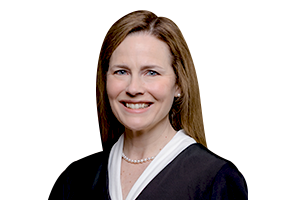
\includegraphics[width=1.5cm]{Figures/justice_images/Barrett.png} &
        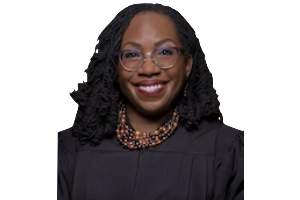
\includegraphics[width=1.5cm]{Figures/justice_images/Jackson.png} \\
        \midrule
    },
    table foot=\bottomrule % Specify the footer rule
]{"Tables/decision_tables/agreement_matrix.csv"}{}%
{ % Process each row
    % Read the content of the first column, append the path and include the image
    \includegraphics[width=1.5cm]{Figures/justice_images/\csvcoli}
    % Print the rest of the columns as they are
    & \csvcolii & \csvcoliii & \csvcoliv & \csvcolv & \csvcolvi & \csvcolvii & \csvcolviii & \csvcolix & \csvcolx
} 
\label{tab:yourlabel}
}
